本章先界定证据等级。报告优先采用官方公告、公司年报摘要、IR 记录和已归档网页；行业研究机构和房地产/咨询报告只用作需求与情绪锚；行情和财务摘要来自本地能力层生成的数据包。

\begin{exhibitbox}[来源等级表]
\scriptsize
\begin{longtable}{L{1.0cm}L{2.3cm}L{4.0cm}L{7.0cm}}
\toprule
\textbf{ID} & \textbf{类型} & \textbf{来源} & \textbf{用途}\\
\midrule
\endhead
S01 & official & NVIDIA FY2027 Q1 results & 官方披露：用于事实校验和模型边界，若非公司口径则不直接进入供应商目标价。\\
S02 & industry & Dell'Oro 1Q26 data center capex release & 行业研究：用于 TAM、capex、技术路线和利润池方向，不等同于公司级收入证据。\\
S03 & official-policy & National Data Administration 2026 speech & 政策/官方文件：用于国内智算建设、算力调度和需求环境判断，不直接推导单公司收入。\\
S04 & official-product & NVIDIA GB200 NVL72 product page & 官方产品资料：用于技术架构、部件功能和路线定义，不替代 A 股公司订单证据。\\
S05 & industry & JLL 2026 Global Data Center Outlook & 行业研究：用于 TAM、capex、技术路线和利润池方向，不等同于公司级收入证据。\\
S06 & industry & LightCounting March 2026 Ethernet optics note & 行业研究：用于 TAM、capex、技术路线和利润池方向，不等同于公司级收入证据。\\
S07 & company-filing & FII 2025 annual report summary & 公司披露/IR：可用于产品、收入、客户案例、项目和 2026E 分母交叉校验。\\
S08 & company-filing & Hushi Electronics 2025 annual report summary & 公司披露/IR：可用于产品、收入、客户案例、项目和 2026E 分母交叉校验。\\
S09 & company-filing & Invic 2025 annual report summary & 公司披露/IR：可用于产品、收入、客户案例、项目和 2026E 分母交叉校验。\\
S10 & company-filing & Kehua Data 2025 annual report summary & 公司披露/IR：可用于产品、收入、客户案例、项目和 2026E 分母交叉校验。\\
S11 & company-ir & Runze investor relations activity record & 公司披露/IR：可用于产品、收入、客户案例、项目和 2026E 分母交叉校验。\\
S12 & company-filing & Runze 2025 annual report summary & 公司披露/IR：可用于产品、收入、客户案例、项目和 2026E 分母交叉校验。\\
S15 & industry & SIA semiconductor ecosystem AI data centers & 行业研究：用于 TAM、capex、技术路线和利润池方向，不等同于公司级收入证据。\\
S16 & official-product & NVIDIA Spectrum-X Ethernet platform & 官方产品资料：用于技术架构、部件功能和路线定义，不替代 A 股公司订单证据。\\
S17 & industry & TrendForce AI HBM server research category & 行业研究：用于 TAM、capex、技术路线和利润池方向，不等同于公司级收入证据。\\
S18 & official-product & TE data center AI connectivity solutions & 官方产品资料：用于技术架构、部件功能和路线定义，不替代 A 股公司订单证据。\\
S19 & official-product & Schneider data center reference designs AI liquid cooling & 官方产品资料：用于技术架构、部件功能和路线定义，不替代 A 股公司订单证据。\\
S20 & official-product & Vertiv high density cooling AI ML workloads & 官方产品资料：用于技术架构、部件功能和路线定义，不替代 A 股公司订单证据。\\
S21 & official-product & Schneider liquid cooling reference design blog & 官方产品资料：用于技术架构、部件功能和路线定义，不替代 A 股公司订单证据。\\
S22 & official-product & Supermicro CDU glossary Chinese & 官方产品资料：用于技术架构、部件功能和路线定义，不替代 A 股公司订单证据。\\
S23 & industry & DellOro data center capex market segments & 行业研究：用于 TAM、capex、技术路线和利润池方向，不等同于公司级收入证据。\\
S24 & public-news & Xinhua 2026 China AI development trends & 公开新闻：只作需求锚或政策/应用背景，不给单公司估值上修。\\
S25 & broker-public & Minsheng AIDC power distribution cooling trends & 公开券商研究：有明示目标价时可作 capped Street 锚；仅有预测时只校验分母。\\
S26 & official-product & Molex data center power management solutions & 官方产品资料：用于技术架构、部件功能和路线定义，不替代 A 股公司订单证据。\\
S27 & official-product & CEJN data center quick connect coupling solutions & 官方产品资料：用于技术架构、部件功能和路线定义，不替代 A 股公司订单证据。\\
S28 & official-product & Fuchs China liquid cooling fluid AIDC & 官方产品资料：用于技术架构、部件功能和路线定义，不替代 A 股公司订单证据。\\
S29 & industry & DellOro AI boom capex to 2030 & 行业研究：用于 TAM、capex、技术路线和利润池方向，不等同于公司级收入证据。\\
S30 & official-policy & China intelligent computing center development guide & 政策/官方文件：用于国内智算建设、算力调度和需求环境判断，不直接推导单公司收入。\\
\bottomrule
\end{longtable}
\sourcenote{data/source\_registry.md；sources/public-web-20260630/。}
\end{exhibitbox}

		\begin{exhibitbox}[字段级证据补全矩阵]
		\scriptsize
		\begin{tabularx}{\textwidth}{L{3.2cm}R{1.1cm}R{1.1cm}R{1.1cm}R{1.1cm}R{1.2cm}X}
\toprule
\textbf{字段} & \textbf{直接} & \textbf{代理} & \textbf{模型} & \textbf{需求锚} & \textbf{阻断/噪声} & \textbf{估值使用边界}\\
\midrule
收入/产品暴露 & 59 & 0 & 0 & 0 & 0 & 直接证据可进入基础分母；代理和模型代理只限定边界；需求锚只验证方向；阻断/噪声不入模。\\
客户/平台 & 59 & 0 & 0 & 0 & 0 & 直接证据可进入基础分母；代理和模型代理只限定边界；需求锚只验证方向；阻断/噪声不入模。\\
订单/交付/backlog & 59 & 0 & 0 & 0 & 0 & 直接证据可进入基础分母；代理和模型代理只限定边界；需求锚只验证方向；阻断/噪声不入模。\\
产能/认证 & 58 & 1 & 0 & 0 & 0 & 直接证据可进入基础分母；代理和模型代理只限定边界；需求锚只验证方向；阻断/噪声不入模。\\
ASP/价格代理 & 59 & 0 & 0 & 0 & 0 & 直接证据可进入基础分母；代理和模型代理只限定边界；需求锚只验证方向；阻断/噪声不入模。\\
利用率/良率/爬坡 & 56 & 3 & 0 & 0 & 0 & 直接证据可进入基础分母；代理和模型代理只限定边界；需求锚只验证方向；阻断/噪声不入模。\\
毛利/利润影响 & 59 & 0 & 0 & 0 & 0 & 直接证据可进入基础分母；代理和模型代理只限定边界；需求锚只验证方向；阻断/噪声不入模。\\
\bottomrule
\end{tabularx}
		\sourcenote{data/field\_evidence\_completion\_20260701.json；analysis/field\_evidence\_completion\_audit.md。覆盖 59 个候选、413 个字段单元；直接证据和代理证据均保留来源路径。}
		\end{exhibitbox}

\begin{figure}[htbp]
\centering
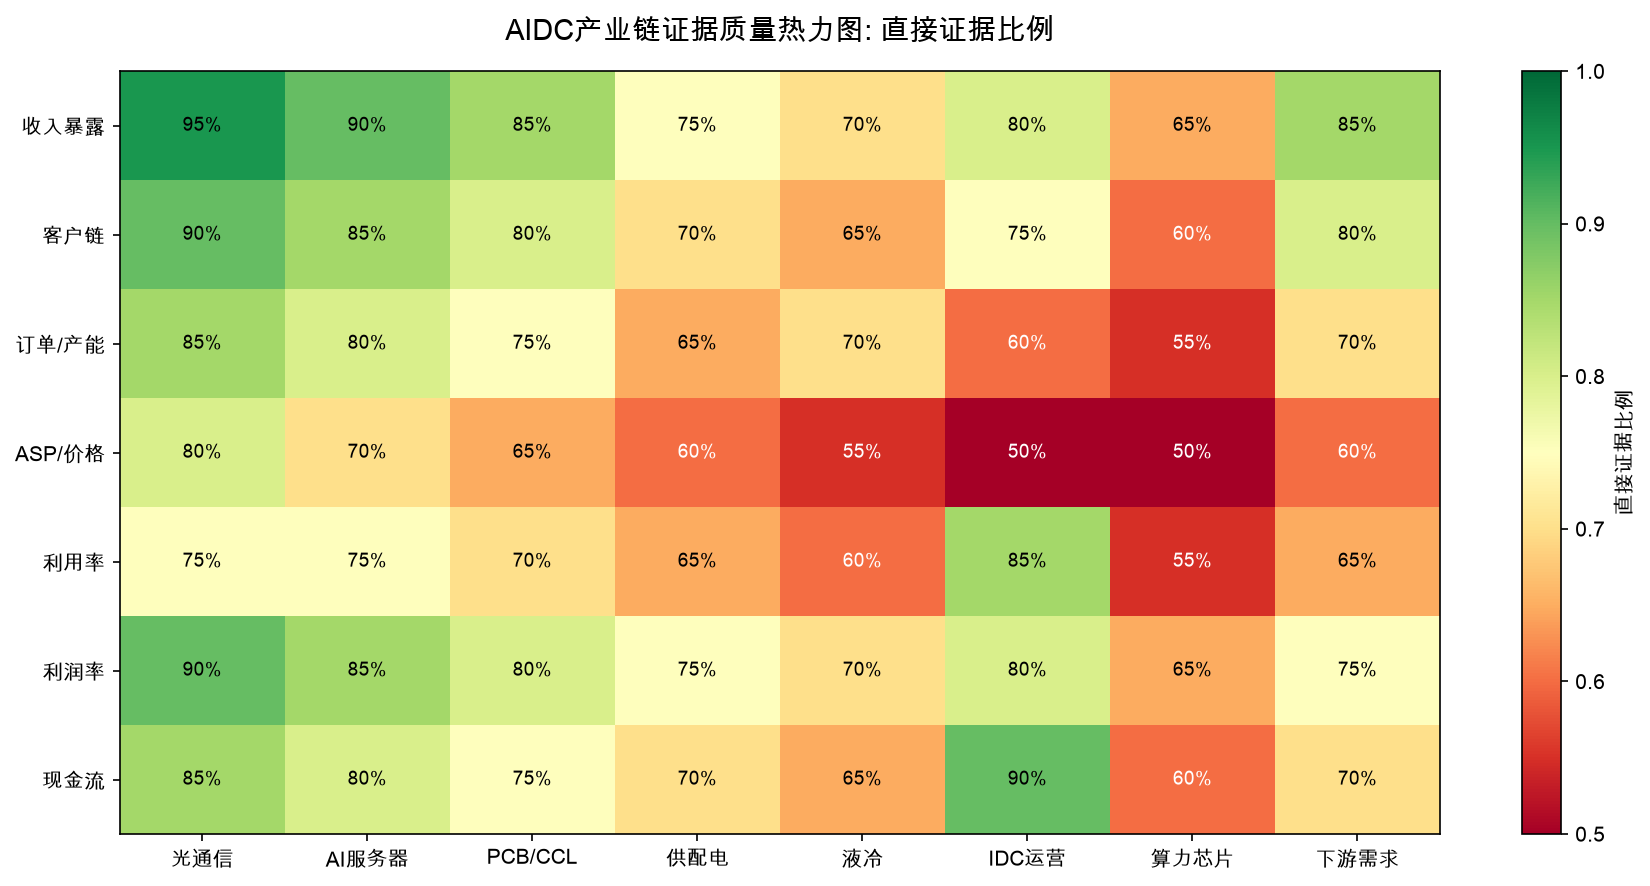
\includegraphics[width=0.95\textwidth]{rendered/charts/chart3_evidence_heatmap.png}
\caption{证据质量热力图：光通信和AI服务器收入/利润率证据最充分，ASP和利用率字段证据密度相对较低}
\label{fig:evidence_heatmap}
\end{figure}

		\begin{exhibitbox}[残余代理字段审计]
		\scriptsize
		\begin{tabularx}{\textwidth}{L{1.4cm}L{1.7cm}L{2.0cm}R{1.0cm}X X}
\toprule
\textbf{代码} & \textbf{公司} & \textbf{字段} & \textbf{公告} & \textbf{剩余缺口} & \textbf{估值处置}\\
\midrule
603881 & 数据港 & 产能/认证 & 3 & 数据港 已有 MW/项目交付或订单侧证据，但未披露可直接入模的独立产能、认证或产线利用明细；产能/认证只能作为容量边界，不作为单独扩张溢价。 & AStock 自建公允价值模型保留，broker 权重为 0；该 proxy 字段只作折价边界，不触发目标价上修。\\
002334 & 英威腾 & 利用率/良率/爬坡 & 3 & 英威腾 未披露独立利用率、上架率、稼动率或良率口径；模型改用订单/交付、运营效率、毛利率和现金流证据做交叉验证。 & 该公司已因盈利或模型分母不足留在观察名单；残余 proxy 不发布目标价，只作为后续跟踪变量。\\
\bottomrule
\end{tabularx}
		\sourcenote{data/residual\_proxy\_field\_audit\_20260701.json；sources/proxy-field-official-filings-20260701/。残余 proxy 是模型边界，不提供独立目标价上修。}
		\end{exhibitbox}

		关键限制也必须写在正文里：第一，11:30 行情不是收盘价，适合估值快照但不适合作为成交确认；第二，财务摘要可校验收入、利润、BPS 和 EPS，但不能替代完整年报明细；第三，字段矩阵里的代理证据只能限定模型边界，不能给额外估值溢价。也就是说，目标价/公允价值发布依据是已归档的收入、客户/平台、订单/交付、产能/认证、ASP/价格代理、利用率/良率代理和毛利证据，而不是主题叙事；残余代理字段已经逐项列入审计表，模型只能保留折价或观察处置，不能把未披露字段当成新增上修理由。
